\chapter{Results}

\section{Simulated Data}

\subsection{Test Cases}

The test cases looked at were selected to determine the effects of the spacecraft inertia, the spacecrafts orbit and its geometry. In Total 18 total cases were simulated, each at multiple different time of the year and multiple random angular velocities.

The geometries used in this analysis were a rectangular prism, a cylinder, and a box-wing. The first two are convex geometries that have differing levels of symmetry, while the box-wing geometry is concave. The orbits examined are low, medium and geostationary Earth orbits. The final variable is the spacecrafts inertia. In the first case, the pricipal inertial axes are assumed to be aligned with the spacecraft body frame and equal. The effect of this is to make the spin axis constant for all time. In the second case, the principal inertial axes are all different and are not aligned with the body frame, causing the spin axis to change over time.

\begin{figure}\label{simulated_geometries}
	\begin{tabular}{cc}
		\includegraphics[width = 65mm]{Long_Rectangle_Image.png} &
		\includegraphics[width=65mm]{Cylinder_Image} \\
		Rectangular Prism & Cylinder \\
		\multicolumn{2}{c}{\includegraphics[width=65mm]{Box_Wing_Image}} \\
		\multicolumn{2}{c}{Box Wing}
	\end{tabular}
	\caption{Three Simulated Geometries.}
\end{figure}


\begin{figure}
	\begin{tabular}{cc}
		\includegraphics[width = 65mm]{leo_orbit} &
		\includegraphics[width=65mm]{meo_orbit} \\
		Low Earth Orbit & Medium Earth Orbit \\
		\multicolumn{2}{c}{\includegraphics[width=65mm]{geo_orbit}} \\
		\multicolumn{2}{c}{Geostationary Orbit}
	\end{tabular}
	\caption{Three Simulated Orbits.}
\end{figure}

\subsection{Simulation Methodology}

First, a LEO, MEO, and GEO orbit were selected. Passes were calculated by brute force sampling a spacecrafts location and checking for necessary conditions. These conditions were obviously that the spacecraft must be above the horizon of the observation site and that the spacecraft be illuminated. Passes lower than 20 degrees elevation were discarded. Additionally, in preliminary experiments it was noticed that the UKF often failed to converge to a solution when the solar phase angle (SPA) was greater than 90 degrees. Therefore passes with an SPA greater than 90 degrees were also discarded. Passes were also limited to only 5 minutes of data collection as MEO spacecraft passes can be hours long and geostationary passes are of course perpetual.

Once a pass was identified, the spacecraft was given three initial attitudes and angular velocities between 0.1 and 0.3 radians per second. These were then propagated and used to calculate three different light curves per pass. Before entering the Kalman Filter, Gaussian noise was added to the light curve whose distribution was similar to that of the real data collected.
\subsection{Simulation Results}

The simulation results reveal that the problem of uniquely identifying an attitude profile from a light curve is an indeterminate problem. The data shows that for any light curve, there are multiple combinations of attitude profiles and angular velocities that can produce it. Many of these solutions are a result of the symmetry of the spacecraft. For example, a rectangular prism rotated by 180 degrees about any axis will appear indistinguishable from its original orientation assuming that each face has identical reflectance properties.

Another source of indeterminacy comes from the truth that it is impossible to distinguish between an object rotating about an axis clockwise and counterclockwise. Therefore, in this thesis, only the axis of rotation is examined. What this means is that, during analysis, the estimated angular velocity was multiplied by 1 or -1 to minimize the dot product between the true angular velocity and estimated angular velocity. This simply serves to make valid results more apparent.

This thesis defined a successful run to one in which a stable solution was converged upon which closely matched the data.  In the trails where the angular velocity was held constant, the metric for a stable solution was the standard deviation of each component of the angular velocity. Once a solution was found, it was noticed that the variance of the rate estimates shrank rapidly. The threshold of standard deviation used in this thesis was 1e-4 radians/second. Determining convergence is not always so simple however, and so a few rare exceptions were identified by hand to have converged to a valid solution despite violating the threshold.

Angular velocities were analyzed in two frames: The body frame and the observation frame. The body frame is the refference frame fixed to the spacecraft body. In this frame, direct comparisons can be made to the ground truth, however it does not account for alternate orientations resulting in the same light curve. 

In order to compare the estimated angular velocity with the truth the observation frame is used. The observation frame is defined to have its origin at the center of the spacecraft, its X axis along the observation vector, the Z axis being the cross of the sun and observation vector, and the Y axis completing the frame. 

This frame enabled comparisons between the estimated and true angular velocities in a frame which is irrespective of the spacecrafts attitude. Additionally, this frame allows for the results of this thesis (which show that some additional solutions exists which are mirrored about the observational plane) to be more easily visualized.

It can be noticed in the formulation of the measurement model that measured light intensity is a function of the relative directions of the facet normals, observation, and velocity vectors. Therefore, if one imagines a mirror floating beneath the spacecraft in the observation plane (The XY plane of the observation frame), it can be visualized that it would result in an identical lightcurve.

This is only possible when the observational plane remains relatively constant however. As the observational plane changes, so must the mirrored angular velocity. As the UKF used in this thesis assumes that the angular velocity is either constant or changes according to Eulers equations of rigid body motion. This unmodeled motion usually excludes the mirrored solution as valid.

%include plot of the OBSERVATION frame

\subsubsection{The Cylinder}

A total of 117 simulations were run using the cylinder geometry. These simulations were roughly evenly distributed across LEO, MEO, and GEO orbits and roughly half assumed a fixed spin axis.

Using the threshold method dsicussed previously, the UKF converged in 53\% of the LEO trials, in 56\% of the MEO trials, and 65\% of the GEO trials. This is likely due to the fact that in both MEO and LEO, the amplitude of the light curve can vary dramatically across the pass as the objects distance from the observer changes. This means that small errors in the state estimate correspond to different magnitude errors depending on when they occur during the pass.  is to say that the model uncertainty changes throughout the pass while the UKF assumes it is constant. The reason MEO performs better than LEO is because a MEO object near apogee has a very constant amplitude. GEO effectively do not change their distance from the observer and so their model uncertainty remains extremely constant.

%Insert bar chart of the differences in convergence

Since a cylinder is symmetrical about its long axis, it is expected that the angular velocity along this axis be the hardest to determine. A perfectly uniform cylinder looks no different while completely stationary than it does spinning about its long axis. Angular velocity about the transverse axes are expected to be much more easily determined. This matches with the results of this thesis. The mean error about the X axis was 5.46E-2 rad/s, the Y axis 6.10E-2 and the Z axis was 1.06E-1. The X and Y body axes error were almost identical while the Z axis was significantly worse.

\begin{figure}[ht]
	\begin{center}
		\begin{tabular}{| c | c | c |}
			\hline X-Axis & Y-Axis & Z-Axis \\ 
			\hline $5.46\times 10^{-2}$ & $6.10\times 10^{-2}$ & $1.06\times 10^{-1}$ \\
			\hline
		\end{tabular}
	\end{center}
	\caption{Mean Errors in the Body Frame for the Cylinder Geometry}
\end{figure}

In figure \ref{simulated_geometries} it can be seen that the cylinder model is modeled as a set of flat facets. It is likely that as the number of facets increases that the error along the Z axis also increases. This is because as the cylinder rotates each facet bightens and then dims, creating a low bumps in the intensity signal that would not be caused by a true cylinder. These "bumps" very likely make it easier for the UKF to converge on the Z axis angular velocity.

In the observation frame, it was observed that of the converged trials, the angular velocity was most accurate about the Z axis of the observation frame. This makes sense because an error along this axis would affect the directions of both the sun and observation vector with respect to the body. 

\begin{figure}[ht]
\begin{center}
\begin{tabular}{| c | c | c |}
	\hline X-Axis & Y-Axis & Z-Axis \\ 
	\hline $1.35\times 10^{-2}$ & $1.37\times 10^{-2}$ & $2.41\times 10^{-4}$ \\
	\hline
\end{tabular}
\end{center}
\caption{Mean Errors in the Observation Frame for the Cylinder Geometry}
\end{figure}


The results were that along the Z axis of the observational frame, the mean error was $2.41\times 10^{-4}$ while along the X and Y axes they were $1.35\times 10^{-2}$ and $1.37\times 10^{-2}$ radians/second respectively.

By examining the angular velocities in the observation frame, it was observed that 6 of the 117 trials converged to a solution which was mirrored across the observational plane. This was apparent because the angular velocity converged to the correct axis and magnitude with the exception that the Z component was the negative of what the truth.




\section{Real Data}

\subsection{SERT-2}

The Space Electric Rocket Test II (SERT-2) is a modified Aegena rocket body whose mission was to test two ion propulsion systems on board. \cite{sert2} In order to power these propulsion systems, two deployable solar panels were added to the Aegena rocket body whose dimensions were 1.5x6 meters. The dimensions of the Aegena module were also 1.53x6 meters.

SERT-2 was launched on February 3rd, 1970 and was finally decommissioned in 1991. Due to the age of the spacecraft and considering that there is potentially fuel remaining within the Aegena tank, this spacecraft can be assumed to be spinning about its major axis. This obviously simplifies the UKF model and allows this thesis to implement the simpler version.

The geometry of SERT-2 is essentially a cylinder with two rectangular panels radiating from one end. This model is non-convex which means that it can take advantage of ray tracing algorithm described in this thesis. 

\begin{figure}
	\begin{tabular}{cc}
	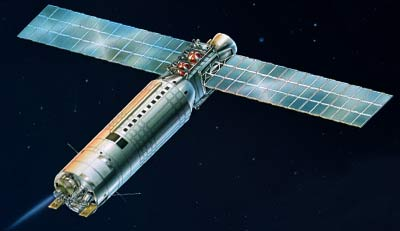
\includegraphics[width = 80mm]{figures/sert-2} & \includegraphics[width = 60mm]{figures/SERT2_Image} \\
	SERT-2, Source: NASA & SERT-2 Reflectance Model 
	
	\end{tabular}
	\caption{SERT-2 vs Reflectance Model}
\end{figure}


\subsection{Ajisai (EGS)}

Ajisai was a mission launched on August 13th, 1986 and was primarily intended as a dummy payload for the H-I launch vehicle. \cite{ajisai_jaxa} Ajisai is essentially a sphere covered with 1,436 corner cube reflectors and 318 mirrors. \cite{ajisai} Its secondary mission (after being mass) was to determine the exact position of the more isolated Japanese islands. \cite{ajisai_jaxa}

Because this spacecraft is so old and because it is a sphere. It is highly likely that it is spinning about its major axis and the simpler UKF formulation can be applied once more.

\begin{figure}
	\begin{tabular}{cc}
	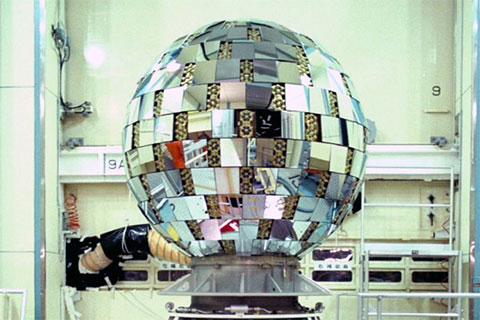
\includegraphics[width = 90mm]{figures/ajisai.jpg} & \includegraphics[width = 60mm]{figures/AJISAI} \\
	AJISAI, Source: JAXA & AJISAI Reflectance Model
	\end{tabular}
	\caption{AJISAI vs Reflectance Model}
\end{figure}

The geometry of the spacecraft is simply a large set of reflective panels. Being mirrors, these panels will have very high specular reflectance and almost no diffuse reflectance. The corner cube reflectors designed to reflect light back to its source. For this thesis, that source is the sun, and so the corner cube reflectors can be assumed to contribute nothing to the lightcurve. Thankfully, the positions of each corner cube reflector were documented, and the panel locations can be inferred from them.

\begin{figure}
	\centering
	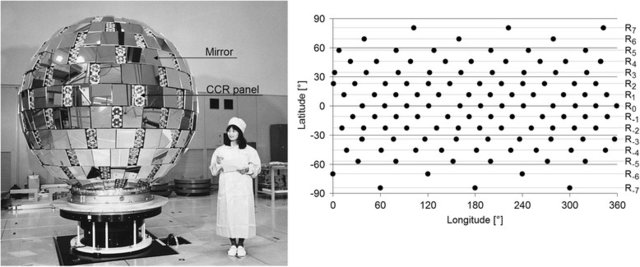
\includegraphics[width = 150mm]{figures/ajisai_panels.jpg}
	\caption{Ajisai with Engineer [Left]. Corner Cube Reflector Locations [Right] \cite{ajisai}}
\end{figure}

\section{Symmetrical Solution Groups}